%% BioMed_Central_Tex_Template_v1.06
%%                                      %
%  bmc_article.tex            ver: 1.06 %
%                                       %

%%IMPORTANT: do not delete the first line of this template
%%It must be present to enable the BMC Submission system to
%%recognise this template!!

%%%%%%%%%%%%%%%%%%%%%%%%%%%%%%%%%%%%%%%%%
%%                                     %%
%%  LaTeX template for BioMed Central  %%
%%     journal article submissions     %%
%%                                     %%
%%          <8 June 2012>              %%
%%                                     %%
%%                                     %%
%%%%%%%%%%%%%%%%%%%%%%%%%%%%%%%%%%%%%%%%%


%%%%%%%%%%%%%%%%%%%%%%%%%%%%%%%%%%%%%%%%%%%%%%%%%%%%%%%%%%%%%%%%%%%%%
%%                                                                 %%
%% For instructions on how to fill out this Tex template           %%
%% document please refer to Readme.html and the instructions for   %%
%% authors page on the biomed central website                      %%
%% http://www.biomedcentral.com/info/authors/                      %%
%%                                                                 %%
%% Please do not use \input{...} to include other tex files.       %%
%% Submit your LaTeX manuscript as one .tex document.              %%
%%                                                                 %%
%% All additional figures and files should be attached             %%
%% separately and not embedded in the \TeX\ document itself.       %%
%%                                                                 %%
%% BioMed Central currently use the MikTex distribution of         %%
%% TeX for Windows) of TeX and LaTeX.  This is available from      %%
%% http://www.miktex.org                                           %%
%%                                                                 %%
%%%%%%%%%%%%%%%%%%%%%%%%%%%%%%%%%%%%%%%%%%%%%%%%%%%%%%%%%%%%%%%%%%%%%

%%% additional documentclass options:
%  [doublespacing]
%  [linenumbers]   - put the line numbers on margins

%%% loading packages, author definitions

\documentclass[twocolumn]{bmcart}% uncomment this for twocolumn layout and comment line below
%\documentclass{bmcart}

%%% Load packages
\usepackage{amsthm,amsmath}
\usepackage{siunitx}
\usepackage{mfirstuc}
%\RequirePackage{natbib}
\usepackage[colorinlistoftodos]{todonotes}
\RequirePackage{hyperref}
\usepackage[utf8]{inputenc} %unicode support
%\usepackage[applemac]{inputenc} %applemac support if unicode package fails
%\usepackage[latin1]{inputenc} %UNIX support if unicode package fails
\usepackage[htt]{hyphenat}

\usepackage{array}
\newcolumntype{L}[1]{>{\raggedright\let\newline\\\arraybackslash\hspace{0pt}}p{#1}}

%%%%%%%%%%%%%%%%%%%%%%%%%%%%%%%%%%%%%%%%%%%%%%%%%
%%                                             %%
%%  If you wish to display your graphics for   %%
%%  your own use using includegraphic or       %%
%%  includegraphics, then comment out the      %%
%%  following two lines of code.               %%
%%  NB: These line *must* be included when     %%
%%  submitting to BMC.                         %%
%%  All figure files must be submitted as      %%
%%  separate graphics through the BMC          %%
%%  submission process, not included in the    %%
%%  submitted article.                         %%
%%                                             %%
%%%%%%%%%%%%%%%%%%%%%%%%%%%%%%%%%%%%%%%%%%%%%%%%%


%\def\includegraphic{}
%\def\includegraphics{}

%%% Put your definitions there:
\startlocaldefs
\endlocaldefs


%%% Begin ...
\begin{document}

%%% Start of article front matter
\begin{frontmatter}

\begin{fmbox}
\dochead{Report from 2015 OHBM Hackathon (HI)}

%%%%%%%%%%%%%%%%%%%%%%%%%%%%%%%%%%%%%%%%%%%%%%
%%                                          %%
%% Enter the title of your article here     %%
%%                                          %%
%%%%%%%%%%%%%%%%%%%%%%%%%%%%%%%%%%%%%%%%%%%%%%

\title{Nipype interfaces in CBRAIN}
\vskip2ex
\projectURL{Project URL: \url{http://cbrain.mcgill.ca}}

\author[
addressref={aff1, aff2},
corref={aff1},
email={tristan.glatard@mcgill.ca}
]{\inits{TG} \fnm{Tristan} \snm{Glatard}}
\author[
addressref={aff1},
%
email={samir.das@mcgill.ca}
]{\inits{SD} \fnm{Samir} \snm{Das}}
\author[
addressref={aff1},
%
email={reza.adalat@mcgill.ca}
]{\inits{RA} \fnm{Reza} \snm{Adalat}}
\author[
addressref={aff1},
%
email={natacha.beck@mcgill.ca}
]{\inits{NB} \fnm{Natacha} \snm{Beck}}
\author[
addressref={aff1},
%
email={remi.bernard@mail.mcgill.ca}
]{\inits{RB} \fnm{Rémi} \snm{Bernard}}
\author[
addressref={aff1},
%
email={najmeh.khalili@mcgill.ca}
]{\inits{NKM} \fnm{Najmeh} \snm{Khalili-Mahani}}
\author[
addressref={aff1},
%
email={pierre.rioux@mcgill.ca}
]{\inits{PR} \fnm{Pierre} \snm{Rioux}}
\author[
addressref={aff1},
%
email={marc.rousseau@mcgill.ca}
]{\inits{MER} \fnm{Marc-Étienne} \snm{Rousseau}}
\author[
addressref={aff1},
%
email={alan.evans@mcgill.ca}
]{\inits{ACE} \fnm{Alan C.} \snm{Evans}}

%%%%%%%%%%%%%%%%%%%%%%%%%%%%%%%%%%%%%%%%%%%%%%
%%                                          %%
%% Enter the authors' addresses here        %%
%%                                          %%
%% Repeat \address commands as much as      %%
%% required.                                %%
%%                                          %%
%%%%%%%%%%%%%%%%%%%%%%%%%%%%%%%%%%%%%%%%%%%%%%

\address[id=aff1]{%
  \orgname{McGill Centre for Integrative Neuroscience (MCIN), Ludmer Centre for
Neuroinformatics and Mental Health, Montreal Neurological Institute
(MNI), McGill University},
  \city{Montréal},
  \street{3801 University Street, WB-208},
  \postcode{H3A 2B4},
  \postcode{Québec},
  \cny{Canada}
}
\address[id=aff2]{%
  \orgname{University of Lyon, CNRS, INSERM, CREATIS.},
  \city{Villeurbanne},
  \street{7, avenue Jean Capelle},
  \postcode{69621},
  %
  \cny{France}
}

%%%%%%%%%%%%%%%%%%%%%%%%%%%%%%%%%%%%%%%%%%%%%%
%%                                          %%
%% Enter short notes here                   %%
%%                                          %%
%% Short notes will be after addresses      %%
%% on first page.                           %%
%%                                          %%
%%%%%%%%%%%%%%%%%%%%%%%%%%%%%%%%%%%%%%%%%%%%%%

\begin{artnotes}
\end{artnotes}

%\end{fmbox}% comment this for two column layout

%%%%%%%%%%%%%%%%%%%%%%%%%%%%%%%%%%%%%%%%%%%%%%
%%                                          %%
%% The Abstract begins here                 %%
%%                                          %%
%% Please refer to the Instructions for     %%
%% authors on http://www.biomedcentral.com  %%
%% and include the section headings         %%
%% accordingly for your article type.       %%
%%                                          %%
%%%%%%%%%%%%%%%%%%%%%%%%%%%%%%%%%%%%%%%%%%%%%%

%\begin{abstractbox}

%\begin{abstract} % abstract
	
%Blank Abstract

%\end{abstract}



%%%%%%%%%%%%%%%%%%%%%%%%%%%%%%%%%%%%%%%%%%%%%%
%%                                          %%
%% The keywords begin here                  %%
%%                                          %%
%% Put each keyword in separate \kwd{}.     %%
%%                                          %%
%%%%%%%%%%%%%%%%%%%%%%%%%%%%%%%%%%%%%%%%%%%%%%

%\vskip1ex

%\projectURL{\url{http://cbrain.mcgill.ca}}
%\projectURL{http://cbrain.mcgill.ca}

% MSC classifications codes, if any
%\begin{keyword}[class=AMS]
%\kwd[Primary ]{}
%\kwd{}
%\kwd[; secondary ]{}
%\end{keyword}

%\end{abstractbox}
%
\end{fmbox}% uncomment this for twcolumn layout

\end{frontmatter}

%{\sffamily\bfseries\fontsize{10}{12}\selectfont Project URL: \url{http://cbrain.mcgill.ca}}

%%% Import the body from pandoc formatted text
\section{Introduction}\label{introduction}

We aim at the large-scale, automatic sharing of software tools between
neuroimaging processing platforms. During the HBM 2015 Hackathon, we
worked on the export of software tools from the Nipype workflow engine
\cite{Gorgolewski2011} to the CBRAIN web platform for distributed
computing \cite{sherif2014cbrain}. Our solution allows to export Nipype
interfaces to the ``Boutiques'' description format importable by CBRAIN
and pointing to a Docker image containing the implementation of the
interface. The interface and its implementation can be automatically
exported from Nipype to CBRAIN (see Fig. 1) and to other platforms
supporting Boutiques (e.g.~Virtual Imaging Platform \cite{GLAT-13} and
the Pegasus workflow engine \cite{DEEL-16}).

\section{Approach}\label{approach}

We developed a tool to export Nipype interfaces to the Boutiques tool
description format (step 1. on Fig 1.). nipype2boutiques relies on
nipype\_cmd, a tool to run Nipype Interfaces as Linux command lines.
nipype2boutiques parses the inputs and outputs of a Nipype interface and
extracts their name, type, description and position on the nipype\_cmd
command line. nipype2boutiques then generates a Boutiques descriptor
pointing to a Docker image where the Nipype interface is available. Once
a Nipype interface is exported using nipye2boutiques, it can be imported
to CBRAIN.

\begin{figure}[h!]
  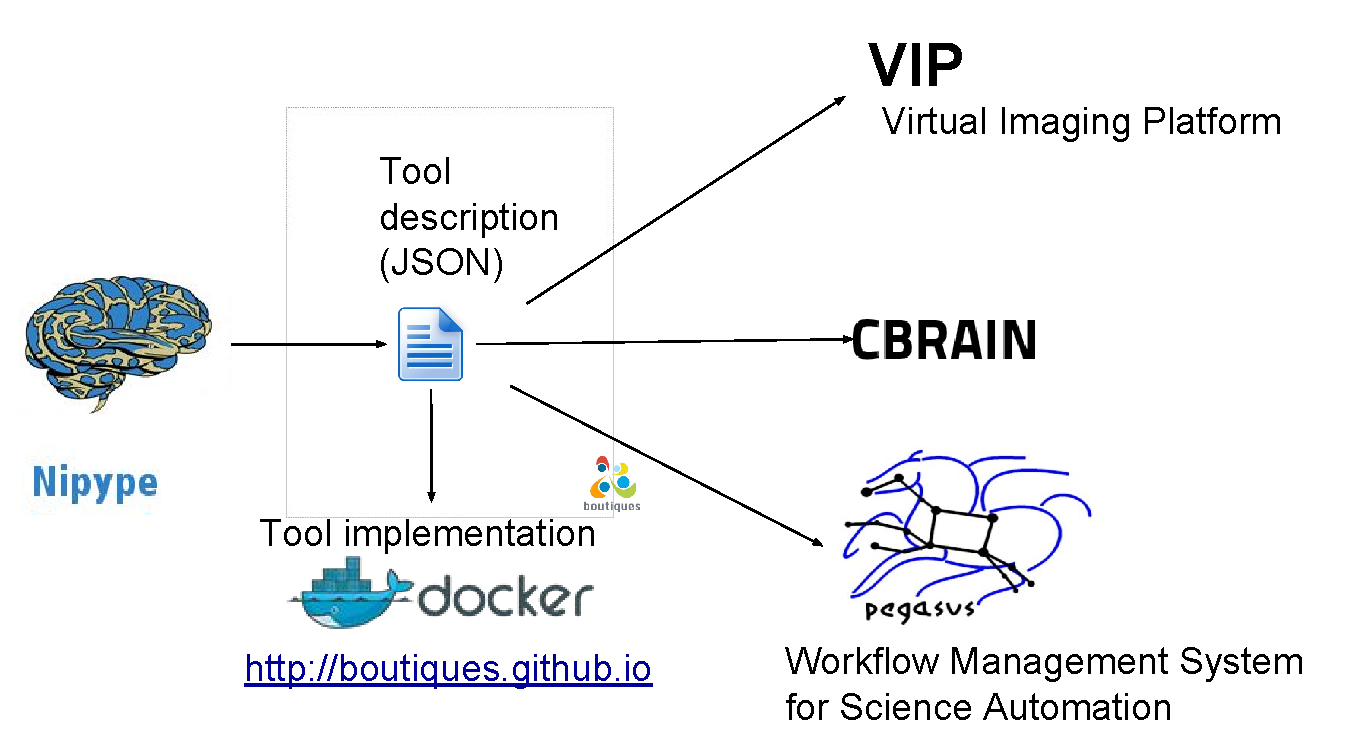
\includegraphics[width=.47\textwidth]{architecture.pdf}
  \caption{\label{centfig} System architecture.}
\end{figure}

\section{Results}\label{results}

We tested nipype2boutiques on a few Nipype interfaces from the FSL
Nipype module. We exported 64 FSL tools automatically from Nipype to
CBRAIN, and made them available at
\url{https://github.com/glatard/boutiques-nipype-fsl}. Limitations
remain on the type of Nipype interface that can be exported by
nipype2boutiques: in particular, InputMultiPath are currently not
supported, and output files have to be written in the execution
directory of the Nipype Interface.

\section{Conclusions}\label{conclusions}

We prototyped a software tool to export Nipype Interfaces as Boutiques
descriptors which can be imported by CBRAIN and other platforms.
Although the solution is still limited to simple interfaces, we believe
that it has the potential to enable fully-automatic tool sharing between
Nipype and CBRAIN.

%%%%%%%%%%%%%%%%%%%%%%%%%%%%%%%%%%%%%%%%%%%%%%
%%                                          %%
%% Backmatter begins here                   %%
%%                                          %%
%%%%%%%%%%%%%%%%%%%%%%%%%%%%%%%%%%%%%%%%%%%%%%

\begin{backmatter}

\section*{Availability of Supporting Data}
More information about this project can be found at: \url{http://cbrain.mcgill.ca}. Further data and files supporting this project are hosted in the \emph{GigaScience} repository REFXXX.

\section*{Competing interests}
None

\section*{Author's contributions}
TG wrote the software and the report; SD contributed to the concept
elaboration at the OHBM event, RA, NB, PR and MER provided support on
the CBRAIN framework, RB implemented Boutiques in CBRAIN, NKM provided
background information on fMRI packages, ACE spearheaded the project.

\section*{Acknowledgements}
The authors would like to thank the organizers and attendees of the 2015
OHBM Hackathon.

  
  
%%%%%%%%%%%%%%%%%%%%%%%%%%%%%%%%%%%%%%%%%%%%%%%%%%%%%%%%%%%%%
%%                  The Bibliography                       %%
%%                                                         %%
%%  Bmc_mathpys.bst  will be used to                       %%
%%  create a .BBL file for submission.                     %%
%%  After submission of the .TEX file,                     %%
%%  you will be prompted to submit your .BBL file.         %%
%%                                                         %%
%%                                                         %%
%%  Note that the displayed Bibliography will not          %%
%%  necessarily be rendered by Latex exactly as specified  %%
%%  in the online Instructions for Authors.                %%
%%                                                         %%
%%%%%%%%%%%%%%%%%%%%%%%%%%%%%%%%%%%%%%%%%%%%%%%%%%%%%%%%%%%%%

% if your bibliography is in bibtex format, use those commands:
\bibliographystyle{bmc-mathphys} % Style BST file
\bibliography{brainhack-report} % Bibliography file (usually '*.bib' )

\end{backmatter}
\end{document}
